\lstset{language=Java, numbers=left, numberstyle=\tiny, stepnumber=2, numbersep=5pt}
\chapter{Introduction}
\label{intro}
In today's world, where increasingly large amounts of data have to be processed and exchanged by distributed systems, the requirements for communication between distributed systems are becoming more and more complex. Not only performance is a problem, but also the requirement to make the services of the distributed systems available to several users at the same time. In other words, every system that is part of the architecture of a distributed system must be able to communicate with every other subsystem at the same time.\\
There are several technologies in the Java environment that can be used for communication within such a distributed system. The most basic variant is the use of Java Sockets. But this assignment favors the Java Remote Method Invocation. This report considers both technologies and presents a possible solution for a distributed system in which both of them play a role.
%%%%%%%%%%%%%%%%%%%%%%%%%%%%%%%%%%%%%%%%%%%%%%%%%%%%%%%%%%%%%%%%%%%%%%%%%%%%%%%%%%%%%%%%%%%%%%%%%%%%%%%%%
%%%%%%%%%%%%%%%%%%%%%%%%%%%%%%%%%%%%%%%%%%%%%%%%%%%%%%%%%%%%%%%%%%%%%%%%%%%%%%%%%%%%%%%%%%%%%%%%%%%%%%%%%
%%%%%%%%%%%%%%%%%%%%%%%%%%%%%%%%%%%%%%%%%%%%%%%%%%%%%%%%%%%%%%%%%%%%%%%%%%%%%%%%%%%%%%%%%%%%%%%%%%%%%%%%%
\chapter{Network Programming in Java}
\label{network-programming}
This chapter explains the theoretical basis for this assignment. The first section focuses on Java sockets, while the second deals with Remote Method Invocation (RMI). The aim is to highlight the differences as well as the advantages and disadvantages of both technologies.
\section{Sockets in Java}
A socket is an endpoint of a bi-directional communication connection between two programs running in different processes on the same computer or on different computers in a network . One socket takes on the role of the server, while the second socket acts as a client. Socket classes are used in Java to represent the connection between a client program and a server program. Sockets provide a simple API and require a hostname and a free port number to be initialized. If two or more sockets are running on the same computer, the hostnames and portnumbers must be different. Before the two processes (no matter if they are running on different computers or not) can communicate with each other, the client and server sockets must perform two different tasks.
\\
First of all, the client must know the hostname and port number of the server in order to connect to it. How exactly this is done depends on the programmer's decision. The server's address data can be stored permanently in the client's program code or can be retrieved by other techniques such as DNS. When establishing a connection between client and server, the client must also identify itself by sending its own host address to the server. The only thing the server has to do is to listen to possible clients attempting to open a connection.
\\
After the connection has been established, data can be transferred in both directions between server and client. The next two chapters show two different socket types and their differences.
\subsection{TCP Socket}
In general there are two different socket types. The first is the \textbf{Stream Socket} whose communication is based on the Transmission Control Protocol (\textbf{TCP}). Because TCP is connection oriented, the Three-Way-Handshake routine must be performed between server and client. This ensures a stable connection between the two end points via which data can be transmitted. TCP also has a built-in error recovery routine which automatically detects and attempts to fix connection terminations, lost data packets and other failures. The main advantage of this kind of socket is that the communication is safer, because lost packets are detected and resent by the sender (server or client). The main disadvantage is, that these sockets have a larger overhead with the complicated connection establishment and error recovery routines and are therefor slower. Figure \ref{tcpsocket} shows the necessary function calls, both Stream sockets must perform to establish a connection and transmit data:\\
\begin{figure}[H]
	\centering
	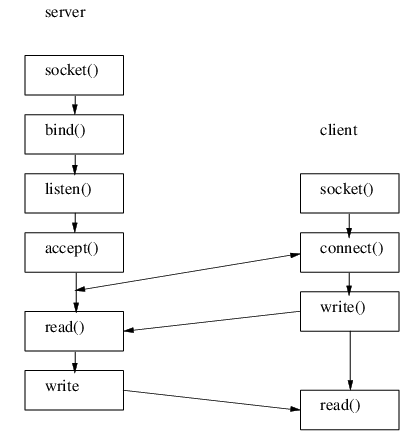
\includegraphics[width =0.7\textwidth]{tcpsocket.PNG}
	\caption{TCP communication between server and client}
	\label{tcpsocket}
\end{figure}
\subsection{UDP Socket}
The \textbf{Datagram Socket} is used for \textbf{UDP} (User Datagram Protocol) communication between two endpoints in the network or between two processes on the same computer.
\\Unlike TCP, UDP does not work connection-oriented. Here the transmitter sends its packets to the destination without worrying about whether the destination is reachable at all. There is also no error recovery because the sender doesn't care if its packets get lost or not. Datagram sockets are only used in certain use cases. Normally, the sender does care whether its packets arrive at their destination or not, which is why this type of communication is rarely used. UDP is only an alternative if the same information is repeated at short intervals, or if the receiver can easily restore missing information using the context. The main advantage however is that UDP is much faster than other network protocols. Figure \ref{udpsocket} shows the function calls both Datagram sockets must perform to transmit data to each other:\\
\begin{figure}[H]
	\centering
	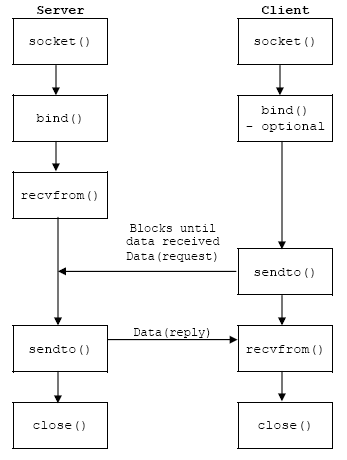
\includegraphics[width =0.6\textwidth]{udpsocket.PNG}
	\caption[Caption for LOF]{UDP communication between server and client\footnotemark}
	\label{udpsocket}
\end{figure}
\footnotetext{image-source: http:///www.tenouk.com//Module41a.html}
\section{Java Remote Method Invocation}
Remote Method Invocation (\textbf{RMI}) enables the call of a method of a remote Java object. The target object is located in another Java virtual machine that can run on a remote or local computer. The call looks exactly like a local call for the calling object, but special exceptions must be caught that can signal connection errors. This technique makes it very easy to build a distributed system in Java, which seems to communicate via normal method calls. For example, RMI can be used to outsource compute-intensive tasks to connected systems that have stronger processors or are simply less busy at the moment. 
\\
Again the basic architecture for RMI is distributed in a client and a server system. The server specifies an interface describing the method or methods that can be called remotely. This interface is called \textit{Remote Interface}. For the client to be able to call a remote method, it must also know this remote interface. The server however must provide a class which implements this interface and therefor provides a real method that can be invoked. This class must also inherit from the \textit{UnicastRemoteObject} class so that the JVM can create stubs and skeletons. The stub is a proxy object, which is required by the client to call the remote method. The skeleton is the proxy of the object on the server side. Figure \ref{rmi} shows RMI's architecture:
\begin{figure}[H]
	\centering
	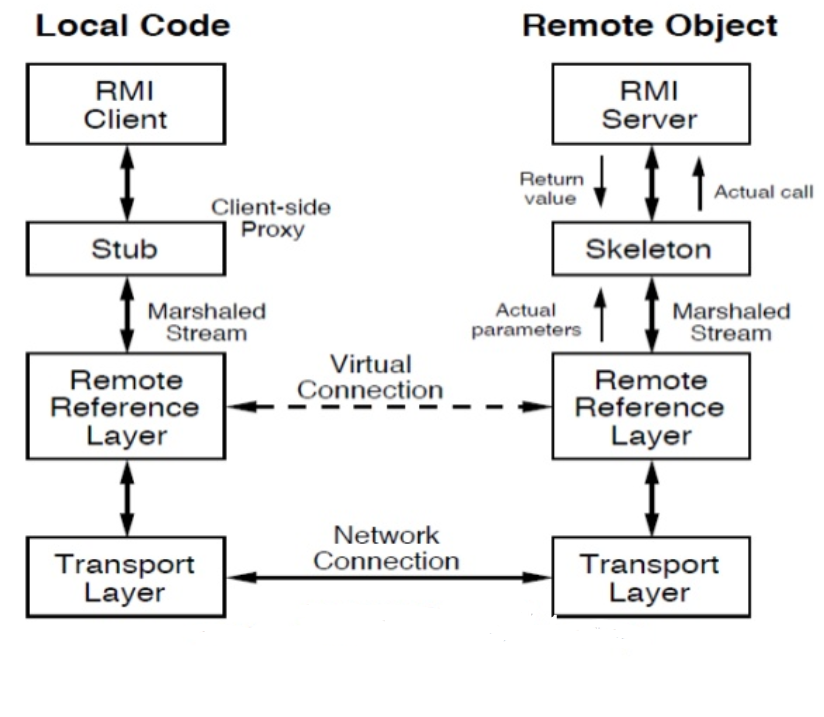
\includegraphics[width =0.8\textwidth]{rmi.png}
	\caption[Caption for LOF]{The RMI architecture\footnotemark}
	\label{rmi}
\end{figure}
\footnotetext{image-source: https://www.slideshare.net/tedionn/java-rmi-26537540}
Because the remote method offers the possibility to pass parameters and return return values to the caller, some additional information has to be considered. It is possible to pass and return simply data types such as integers or strings without taking further action. But if the user wants to transfer complex objects such class-instances, their classes must implement the \textit{Serializable}-Interface.
\\
Parameters can be transferred via \textit{Object by Value} and \textit{Object by Reference}. The first means that a copy of the object is sent from the client to the server or the other way around. In the case of the second, a real reference to the object is transferred.
\\
The remote object (or service object) must be registered in the RMI registry, which is part of the JRMI environment. This is done with a unique name. This is necessary because the client uses this name to retrieve the object reference from this registry and thus obtains access to the service object. The communication between client and server is based on a simple request/reply protocol. This is why only the client can call methods on the server remotely. The other way around isn't possible. All server-methods that can be called remotely must also throw a \textit{RemoteException} if there is a connection error.

\section{Sockets vs RMI}
Both technologies have their own use-cases, advantages and disadvantages. Sockets are completely platform-independent because they are available in any programming language. RMI, on the other hand, is only available in Java. There are similar technologies in WCF in the. NET environment that allow remote method calls. However, they work differently than RMI in Java. The main disadvantage of sockets is that the programmer has to take care of the function calls of the low level APIs and their error handling, which is often a bit cumbersome. The biggest advantage is that sockets produce a very low overhead and are therefore much faster.
\\
As RMI is based on Java Sockets, there are still Sockets doing the work in the background transmitting the data using TCP. However, the programmer does not have to worry about their functionality. This simplicity is the main advantage of RMI over sockets. The main disadvantage is that RMI does not support bidirectional communication. The client is always the one who calls methods of the server. It is not possible the other way around. These method calls also do not work asyncronously. The client must wait for the server's response in the thread where the method call occurred. Sockets however do not have this disadvantage. Here the communication works completely asyncronously. Another drawback when using RMI is the larger communication overhead, since RMI works on a higher level than Sockets. Therefor RMI is slower than the low-level sockets. When comparing the advantages and disadvantages of both, RMI and Sockets, it seems that sockets are more practical because they don't have that many restrictions. But there are still situations, where RMI can be useful because of it's simplicity.
%%%%%%%%%%%%%%%%%%%%%%%%%%%%%%%%%%%%%%%%%%%%%%%%%%%%%%%%%%%%%%%%%%%%%%%%%%%%%%%%%%%%%%%%%%%%%%%%%%%%%%%%%
%%%%%%%%%%%%%%%%%%%%%%%%%%%%%%%%%%%%%%%%%%%%%%%%%%%%%%%%%%%%%%%%%%%%%%%%%%%%%%%%%%%%%%%%%%%%%%%%%%%%%%%%%
%%%%%%%%%%%%%%%%%%%%%%%%%%%%%%%%%%%%%%%%%%%%%%%%%%%%%%%%%%%%%%%%%%%%%%%%%%%%%%%%%%%%%%%%%%%%%%%%%%%%%%%%%
\chapter{Job Server/Client Architecture}
\label{job}
The main part of this report focuses on the design of a distributed client-server architecture using the technologies presented in the previous chapters. Sockets are used to establish a connection between the client and the server, while RMI is used to transfer jobs that the server should process for the client from the client to the server. In this first part, the requirements for this system will be presented:
\begin{itemize}
	\item It shall be possible, that several clients connect several servers at the same time.
	\item A server shall process several jobs at once.
	\item The communication between client and server should be implemented by using RMI.
	\item After starting the client, it should find the server by executing a multicast-lookup.
\end{itemize}
These requirements led to the architecture and functionality shown in the next chapters.
\section{Overall Architecture}
The very first requirement dictates the basic server-client architecture for this project. Every Server must be able to connect to several clients and handle their job-requests at the same time. On the other side every client must be able to connect to several servers at once. So this indicates that multi-threading must be used in the solution in order to paralellize the different tasks of server and client logic so they can work simultaneously. The resulting architecture is shown in Figure \ref{server-client-architecture}.
\begin{figure}[H]
	\centering
	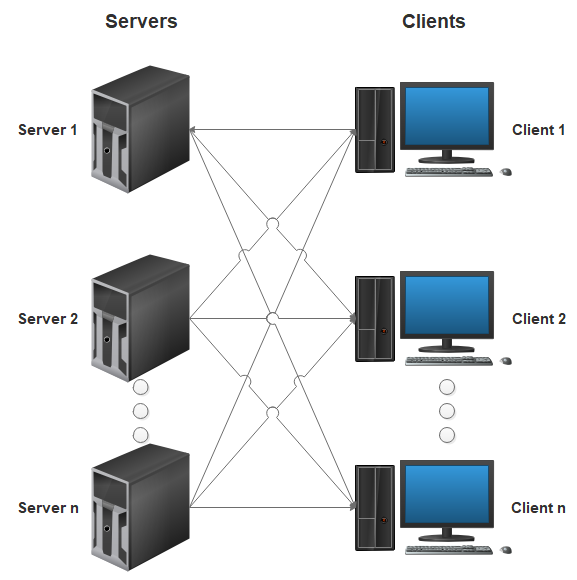
\includegraphics[width =0.7\textwidth]{server-client-architecture.PNG}
	\caption{Basic server-client architecture for the project}
	\label{server-client-architecture}
\end{figure} 

\section{UDP-Multicast}
In order to be able to send a job for the server, the client must first find out the host name, port and server name under which the RMI server was registered on the server computer.\\
For this purpose, the client uses a UDP multicast. In order for that to work the server must use a multicast socket and thus join a multicast group. The client must furthermore know the address of this multicast group and the port on which the multicast socket is running on the server.\\
Now the client uses a datagram socket to send a UDP multicast packet to the multicast group. All servers that have joined the multicast group receive this packet and send the host address, the port and the server name for the RMI server using another UDP packet to the client. In order for this to work concurrently with the other functions, the sockets must run in separate threads on both the client and the server. Figure \ref{udp-multicast} illustrates the idea for the communication:
\begin{figure}[H]
	\centering
	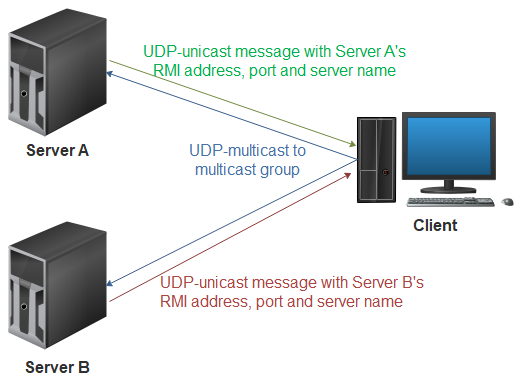
\includegraphics[width =0.8\textwidth]{udp-multicast.PNG}
	\caption{UDP multicast to retrieve the RMI server's information}
	\label{udp-multicast}
\end{figure} 
After the client received multiple replies from multiple servers for his request, it can decide which one should receive the job and send it using the RMI interface and the server's 'contact information'.
\section{The Job Server}
This chapter describes the architecture of the server in detail, while the client is treated as a black box at first.\\
When looking at the requirements, one can see that the server has to perform a lot of tasks at the same time. Thus, multithreading is an important topic. The server should be able to receive multicast messages and send back replies, accept jobs via the RMI interface and process several jobs simultaneously. And all of that at the same time.
\\
To meet these requirements, an architecture has been designed using both sockets and Remote Method Invocation.
\\
First, a class must be introduced that implements the remote interface for the RMI-based communication with the client.This class creates its own RMI registry using an unused port and binds itself to this registry so that it can be found by the client. Instances of that class must run in separate threads so that the server can receive multicast messages from other clients at the same time using a multicast socket. For this purpose another runnable is introduced, which binds this multicast socket to another free port and joins a multicast group. This class also runs in a separate thread to avoid blocking the other functions of the server. After binding, the multicast socket listens for incoming multicast messages.
\\
When a message is received, this 'multicast listener' sends back the host address of the server, the port to which the RMI registry was bound, and the name of the RMI server to the sender of the original message. Now the client has all necessary information to get a reference from the RMI registry of the server to the class that implements the remote interface. The client executes a lookup and gets back a reference from the codebase to the class of the server. The client can now send its job to the server by calling the method on this reference remotely.
\\\\
However, since the server must be able to receive and process several job requests at once, it cannot simply use the same thread to process the job and then return the response. Instead, the server delegates the job to a 'Job Sheduler', which can process multiple jobs at the same time using a thread pool, where each job gets its own thread. As soon as the job is finished, the result is returned to the client. Figure \ref{server-architecture} shows the server's architecture and illustrates the procedures described above.
\begin{figure}[H]
	\centering
	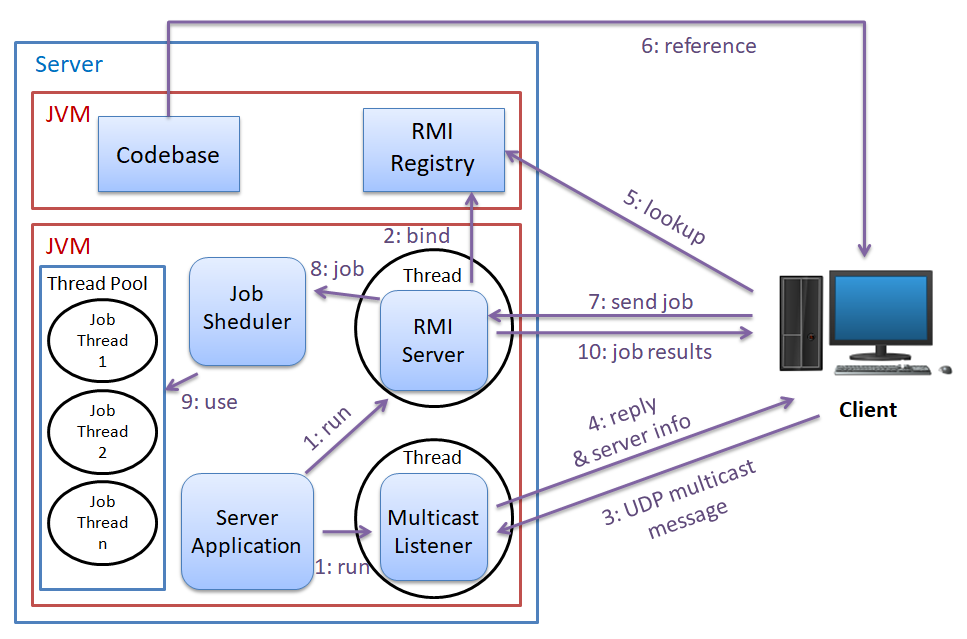
\includegraphics[width =1.0\textwidth]{server-architecture.PNG}
	\caption{Server architecture and necessary calls}
	\label{server-architecture}
\end{figure} 

\section{The Job Client}
This chapter describes the client part of the architecture in detail, while the server explained in the previous chapter is considered here as a black box.\\
The client initially has the problem that it does not have any information about any server. However, in order to be able to forward a job to a server, the client needs its host-address, the port on which the RMI regristry was bound and the name of the RMI server. In order to get this information, the client uses a class which binds a datagram socket to an unused port. This socket is used to send a request at regular intervals to a multicast group to which possible servers are assigned. Now this' multicast sender' must listen to messages that are sent back by servers receiving the multicast message. As shown in the previous chapter, all servers send the required information back to the client as soon as they receive the multicast message.\\
The sender is then stopped and the messages of all servers are evaluated. Since the client must also be able to communicate with several servers at the same time, everything further is executed in parallel. For each received message, a new instance of a runnable class' RMI Client' is created and executed in a new thread, which uses the information from the message to perform a lookup for the server reference on the server machine.\\
As shown in the previous chapter, the RMI registry receives this lookup request and the codebase returns a reference to the target class on the server machine that implements the remote interface. Now the client can call the method on this reference remotely to transmit a job to the server and get the result back as the return value of the method call. Figure \ref{client-architecture} shows the client's architecture as wells as the procedures on the client-side:
\begin{figure}[H]
	\centering
	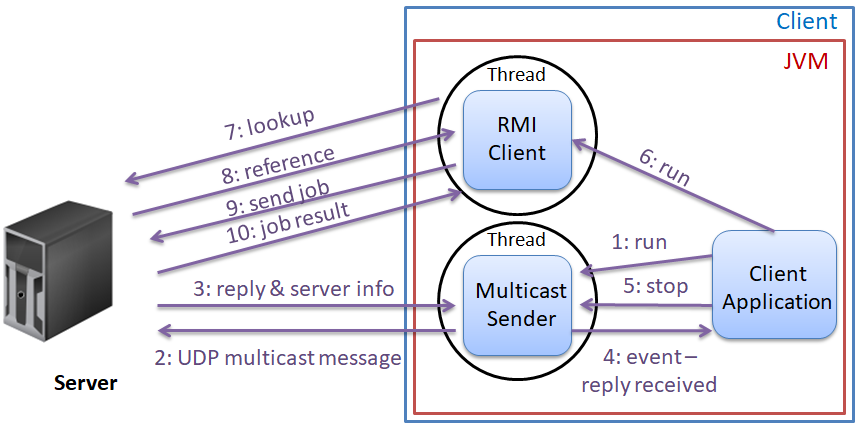
\includegraphics[width =1.0\textwidth]{client-architecture.PNG}
	\caption{Client architecture and necessary calls}
	\label{client-architecture}
\end{figure} 
\section{Load Balancing}
For a large server-client architectur it is important that the same request is not handled by several servers at the same time. This costs resources and is unnecessary because the client only needs a response from one server. At this point, the system should make it possible for the client to send its job request only to one free server that processes the job and sends the result back. In order to optimize the performance, the server that has the lowest load at the time of the request should be selected from all servers. This process is called load balancing.
\\
\\
The load balancing for this architecture should be implemented in the simplest way. Instead of introducing an external load balancer that distributes the incoming requests to the different servers, the load balancing in this system is done directly by client and server themselves.
\\
As explained in the two previous chapters, the server responds to the client's multicast messages by sending its contact information for the RMI Registry and RMI Server back to the client. It also uses a thread pool to process multiple jobs at the same time. In order to realize load balancing in a simple way, the information that the server sends to the client can be extended by additional information. For example, by the number of free threads in the thread pool. Or by the number of currently running job threads. If the client afterwards evaluates this information from several servers, he can very easily select the one with the smallest workload and send his job to that server using RMI. 
\\
This is of course a very simple solution, which has the disadvantage that after receiving the response from a server, the client has to wait for a very short period of time to be able to compare multiple responses from several servers. The advantage is, however, that in this case the server machines are not additionally loaded, since the load balancing takes place on the client. Furthermore, there is no need for a third instance for load balancing, which creates an additional communication overhead, as is the case with most load balancers.
%%%%%%%%%%%%%%%%%%%%%%%%%%%%%%%%%%%%%%%%%%%%%%%%%%%%%%%%%%%%%%%%%%%%%%%%%%%%%%%%%%%%%%%%%%%%%%%%%%%%%%%%%
%%%%%%%%%%%%%%%%%%%%%%%%%%%%%%%%%%%%%%%%%%%%%%%%%%%%%%%%%%%%%%%%%%%%%%%%%%%%%%%%%%%%%%%%%%%%%%%%%%%%%%%%%
%%%%%%%%%%%%%%%%%%%%%%%%%%%%%%%%%%%%%%%%%%%%%%%%%%%%%%%%%%%%%%%%%%%%%%%%%%%%%%%%%%%%%%%%%%%%%%%%%%%%%%%%%
\chapter{Other possible solutions}
\label{other-solutions}
In this chapter, alternative solutions for the architecture of the system are briefly presented and compared with the solutions from the previous chapters.
\section{Using TCP instead of UDP for multicast replies}
An alternative for communication is the use of stream sockets and thus TCP instead of UDP for the server's response to the multicast message from the client. The advantage here would be that communication through TCP is more safe than with UDP. TCP is able to retrieve and resend lost packets (s. chapter \ref{tcpsocket}). This would ensure that the server's response reaches the client. However, since there are several servers in the network, the failure of a response from one server does not cause a severe problem, since there are enough other servers available from which the client can receive a response. Therefore, UDP was favored here instead of TCP in order to benefit from the speed advantage of this protocol (s. \ref{udpsocket}).
\section{Using sockets instead of RMI}
A further alternative for communication would be the complete conversion of communication to sockets. This would mean that one could spare the additional threads for the RMI server and client classes on both the client and the server machine. Another advantage would be that communication via sockets is bi-directional in contrast to communication via RMI. Thus, the same sockets could be used as interfaces for the communication. However, the transfer of objects between server and client would not be as comfortable as it used to be. What was a simple method call with a return value before with RMI would now be much more complex, since the objects that have to be transferred would have to be serialized additionally for the communication via sockets. On the other hand, with sockets there is greater flexibility in communication. So the developer has to decide whether he prefers the simplicity of RMI or the flexibility of sockets.
\section{Load Balancer}
Another alternative implementation option would be to use an additional load balancer for load balancing. The load balancer would receive the multicast messages of the clients and decide from which server to send the RMI information back to the requesting client. There are two different approaches for the load balancer.
\subsection{static load-balancing}
A static load balancer knows the capacity of all servers in the network and, depending on the complexity of the jobs requested by the client, returns the RMI contact information of the most suitable server to the client. Figure \ref{staticloadbalancer} shows a concept for this type of load balancer.
\begin{figure}[H]
	\centering
	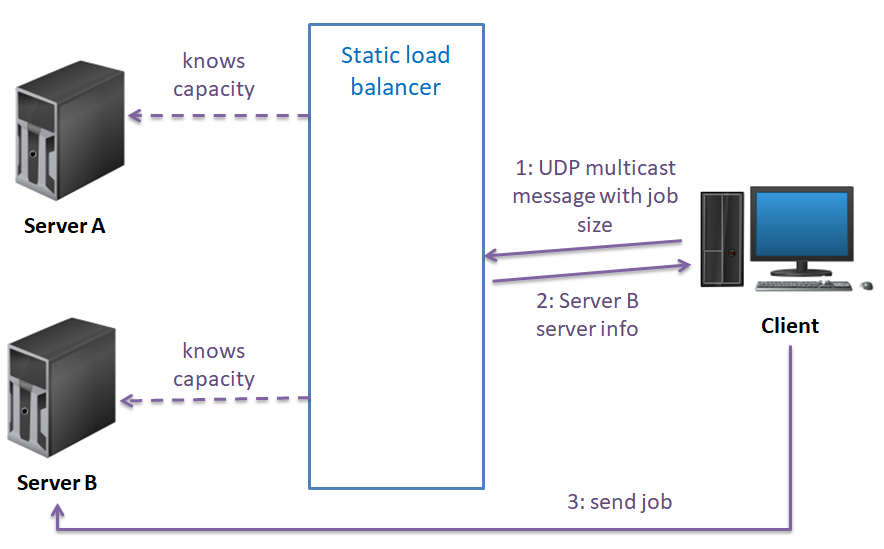
\includegraphics[width =1.0\textwidth]{staticloadbalancer.PNG}
	\caption{Static load balancer}
	\label{staticloadbalancer}
\end{figure} 
This load balancing method is called static, because the load balancer does not care about the current load of each server. It decides only on the basis of the servers' known capacities. This is inefficient in some situations, but the advantage is that it does not generate any unnecessary communication overhead, since the load balancer already has all the necessary information and does not have to request anything from the servers.
\subsection{dynamic load-balancing}
In contrast to the static load balancer, the dynamic load balancer does not have any information about the servers. So it has to request the required information at regular intervals from all servers. Here it requests the current load of each server. If a multicast request from a client arrives at the load balancer, it can return the RMI information of the currently least busy server to the client. Figure \ref{dynamicloadbalancer} shows a concept for this load balancer.
\begin{figure}[H]
	\centering
	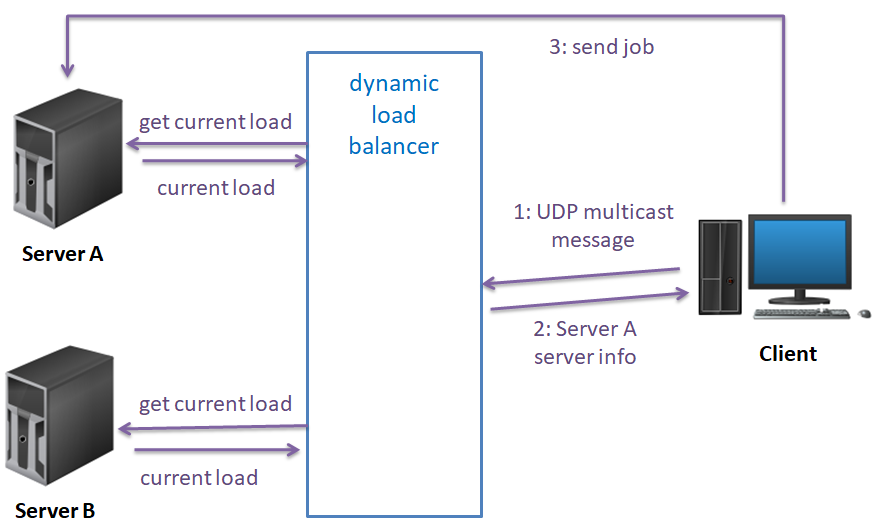
\includegraphics[width =1.0\textwidth]{dynamicloadbalancer.PNG}
	\caption{Dynamic load balancer}
	\label{dynamicloadbalancer}
\end{figure} 
the main advantage here is that the workload is always distributed equally and thus the performance of the system is significantly increased.The disadvantage is that a high network load is generated, because the load balancer must constantly check the current load of all servers.
%%%%%%%%%%%%%%%%%%%%%%%%%%%%%%%%%%%%%%%%%%%%%%%%%%%%%%%%%%%%%%%%%%%%%%%%%%%%%%%%%%%%%%%%%%%%%%%%%%%%%%%%%
%%%%%%%%%%%%%%%%%%%%%%%%%%%%%%%%%%%%%%%%%%%%%%%%%%%%%%%%%%%%%%%%%%%%%%%%%%%%%%%%%%%%%%%%%%%%%%%%%%%%%%%%%
%%%%%%%%%%%%%%%%%%%%%%%%%%%%%%%%%%%%%%%%%%%%%%%%%%%%%%%%%%%%%%%%%%%%%%%%%%%%%%%%%%%%%%%%%%%%%%%%%%%%%%%%%
\chapter{Conclusion}
\label{conclusion}
In this workshop the technology RMI was examined in detail and compared to the classical Java sockets. It has been found that RMI is a very convenient way to implement network communication using java without a lot of effort, so that even complex objects can be transferred without problems. The ability to communicate with a remote system through simple method calls is a huge advantage of RMI over sockets. Nevertheless, sockets do not lose any of their importance and actuality, as RMI does not provide all the possibilities that exist with sockets. This became very clear when examining the implementation possibilities for the given requirements. For example, RMI does not provide functionality for multicasts. Bidirectional communication is also not possible.
\\\\
Another important aspect of this workshop was concurrency and parallelism. As the system had to support several clients as well as several servers, all of which should communicate with each other at the same time, the topic of \textbf{multithreading} could not be overlooked. 
\\\\
Also the topic \textbf{load balancing} was part of this workshop, because it was always the server which had the lowest load that should execute the client's job. For this purpose, several possibilities were presented with the help of which such a system can be implemented in theory.
\\\\
All in all, it can be said that the learning effect in this workshop was very high, as not only different technologies but also different approaches and concepts were used and combined to design an architecture for a distributed system.